%%%%%%%%%%%%%%%
%
% $Autor: Wings $
% $Datum: 2020-01-29 07:55:27Z $
% $Pfad: General/ArduinoCLI.tex
% $Version: 1785 $
%
%
%%%%%%%%%%%%%%%


%@online{ArduinoCLI:2018,
%  publisher = Arduino,
%  year      = 2018,
%  title     = {Arduino CLI 0.33},
%  url = {https://arduino.github.io/arduino-cli/0.33/commands/arduino-cli/}
%}

\chapter{Kammandozeileninterpreter (CLI)}

\textcolor{red}{Quellen für die Bilder fehlen!}

\Mynote{Erklärung von Kammandos in den Anhang}

Seit 2018 bietet die Firma Arduino auch einen Kommandozeileninterpreter an. \cite{ArduinoCLI:2018} Die Web-Version der Entwicklungsumgebung verwendet diese Schnittstelle. Das heißt, alle Funktionalitäten, die die Entwicklungsumgebung zur Verfügung stellt, stehen hier auch zur Verfügung. So kann unter Windows, MacOS und Linux \cite{ArduinoCLI:2022}. Die Entwicklung mit Hilfe des Kommandozeileninterpreters ermöglicht es, wenn konsequent mit Hilfe von Batch-Dateien gearbeitet wird, qualitätssichernde Maßnahmen gezielt durchzuführen. So kann die Konfiguration der Entwicklungsumgebung gesichert und nachvollziehbar wiederholt werden. 


Der Quellcode  kann frei genutzt werden, allerdings muss man bei einer gewerblichen Nutzung eine Lizenz bei der Firma anfragen \cite{ArduinoCLIGit:2022}. Eine ausführliche Dokumentation wird zur Verfügung gestellt. \cite{ArduinoCLIIntro:2020,ArduinoCLIDoc:2022}

Bei der Entwicklung der \ac{cli} stehen drei Aspekte im Fokus. 

\begin{enumerate}
  \item Einerseits ermöglicht die Schnittstelle die Einbettung der Entwicklung in die gewohnte Entwicklungsumgebung. So kann die Schnittstelle auch mit  Edge Impulse\index{Edge Impulse} genutzt werden. 
  \item Zweitens ermöglicht sie die Integration der Entwicklung in die Prozesse Continuous Development\index{Continuous Development} and Continuous Integration\index{Continuous Integration}. Sie ermöglicht damit die Automatisierung der typischen Aktivitäten im Bereich der Softwareentwicklung.
  \item  Des Weiteren ermöglicht es nun die vereinfachte Kommunikation mit Edge Computern, zum Beispiel mit einem Raspberry PI.
\end{enumerate}

\section{Installation und Verwendung des CLI}

Da \ac{cli} ständig weiterentwickelt wird, muss zunächst die aktuelle Version aus dem GitHub-Projekt \url{https://arduino.github.io/arduino-cli/0.32/installation/#latest-release}, siehe \cite{ArduinoCLIGit:2022},  geladen werden. Die hier verwendete Version ist 0.33. \cite{ArduinoCLI:2018}

\bigskip

Nach dem erfolgreichen Download der Datei \FILE{arduino-cli\_0.33.0\_Windows\_64bit.zip} kann der Ordnerinhalt an einen selbst definierten  Speicherpfad extrahiert werden. Die gepackte Datei enthält die Lizenzbestimmungen und die ausführbare Datei \FILE{arduino-cli.exe}. Um die Funktion des Kommandozeileninterpreters in verschiedenen Pfaden nutzen zu können, sollte der Pfad zum Speicherort der Datei \FILE{arduino-cli.exe}  der Systemvariablen \SHELL{PATH} hinzugefügt werden. Anschließend lässt sich das Interface durch die Eingabe \SHELL{arduino-cli} in die Kommandozeile nutzen.


% https://github.com/arduino/arduino-cli#download-the-latest-unstable-alpha-preview.

Nachdem die Installation abgeschlossen ist, kann \SHELL{arduino-cli board list} in der Eingabeaufforderung eingegeben werden. Das angeschlossene Gerät wird als Arduino Portenta H7\index{Portenta H7} mit Portnummer und Typ angezeigt, wie in Abbildung \ref{ArduinoInstallation} dargestellt. Es ist zu beachten, dass die Versionsnummer, hier 0.33.1, gegebenenfalls anzupassen ist. Wenn ein Arduino Nicla Vision\index{Nicla Vision} oder ein Arduino Nano 33 BLE sense \index{Arduino Nano 33 BLE sense}  angeschlossen ist, werden entsprechende Meldungen ausgegeben.

Das Programm \FILE{arduino-cli-0.33.1.windows.exe} wird nun in \FILE{arduino-cli.exe} umbenannt. Daher kann im Folgenden im der Programmname \FILE{arduino-cli.exe} verwendet werden.
    
    
    \begin{figure}
        \centering
        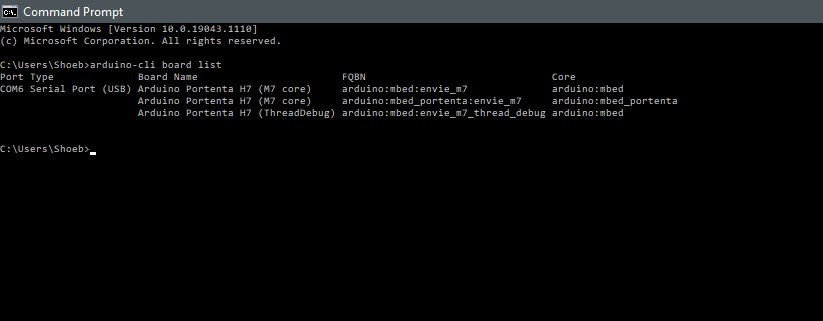
\includegraphics[width=\textwidth]{Arduino/arduino-cli}
        \caption{Installation von Arduino-CLI  }
        \label{ArduinoInstallation}
    \end{figure}


\section{Konfiguration des Arduino CLI}


\URL{https://learn.sparkfun.com/tutorials/efficient-arduino-programming-with-arduino-cli-and-visual-studio-code/introduction-to-the-arduino-cli}

Damit \ac{cli} dir Arduino-Installation finden kann, hilft es, eine Konfigurationsdatei für \ac{cli} zu erstellen. Diese Konfigurationsdatei ist in einem Format YAML\index{YAML} definiert.
Zur Erstellung einer Basis-Konfigurationsdatei kann \ac{cli}  verwendet werden, in dem in einer Kommandozeile 

\medskip

\SHELL{arduino-cli.exe config init}

\medskip

eingegeben wird. Dieser Befehl erstellt eine neue Datei \FILE{.cli-config.yml}. Dort sind alle notwendigen Parameter deklariert. Die Standardeinstellungen der Konfigurationsdatei sind in Abbildung~\ref{KonfigBild} dargestellt. Folgende Parameter müssen in der Regel geändert werden:

\begin{itemize}
    \item \SHELL{sketchbook\_path}: Verzeichnis des Arduino-Sketche. Hier werden alle Bibliotheken und Hardware-Definitionen installiert.
    \item \FILE{arduino\_data}:  Installationsort des Arduino-Boards und des Bibliotheksmanagers. In den meisten Fällen sollte dies nicht geändert werden müssen.
\end{itemize}


Die anderen Optionen können in der Regel auf ihren Standardwerten bleiben.


\begin{figure}
    \begin{center}
        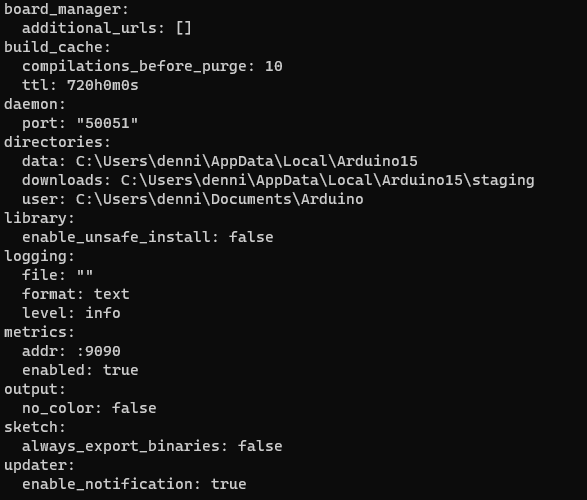
\includegraphics[width=9cm]{Arduino/CLI/StandardConfig.png}
        \caption{Standardeinstellungen der Konfigurationsdatei}
        \label{KonfigBild}
    \end{center}
\end{figure}


\Mynote{Welche Möglichkeiten gibt es in der Konfigurationsdatei?}


\section{Funktionsübersicht}


Die Datei \FILE{README.md} im GitHub-Repository  ``Arduino CLI'' enthält eine hervorragende Übersicht über die Funktionen und Möglichkeiten.\cite{ArduinoCLIGit:2022} 


Folgende Funktionen stehen zur Verfügung \cite{ArduinoCLI:2018}:

\begin{itemize}
  \item \SHELL{arduino-cli}
  \item \SHELL{board}
    \begin{itemize}
      \item \SHELL{board attach}
      \item \SHELL{board details}
      \item \SHELL{board list}
      \item \SHELL{board listall}
      \item \SHELL{board search}
    \end{itemize}
  \item \SHELL{burn-bootloader}
  \item \SHELL{cache}
  \item \SHELL{cache clean}
  \item \SHELL{compile}
  \item \SHELL{completion}
  \item \SHELL{config}
    \begin{itemize}
      \item \SHELL{config dump}
      \item \SHELL{config init}
      \item \SHELL{config add}
      \item \SHELL{config delete}
      \item \SHELL{config remove}
      \item \SHELL{config set}
  \end{itemize}
  \item \SHELL{core}
    \begin{itemize}
      \item \SHELL{core download}
      \item \SHELL{core install}
      \item \SHELL{core list}
      \item \SHELL{core search}
      \item \SHELL{core uninstall}
      \item \SHELL{core update-index}
      \item \SHELL{core upgrade}
    \end{itemize}
  \item \SHELL{daemon}
  \item \SHELL{debug}
  \item \SHELL{lib}
    \begin{itemize}
      \item \SHELL{lib deps}
      \item \SHELL{lib download}
      \item \SHELL{lib examples}
      \item \SHELL{lib install}
      \item \SHELL{lib list}
      \item \SHELL{lib search}
      \item \SHELL{lib uninstall}
      \item \SHELL{lib update-index}
      \item \SHELL{lib upgrade}
    \end{itemize}
  \item \SHELL{monitor}
  \item \SHELL{outdated}
  \item \SHELL{sketch}
    \begin{itemize}
      \item \SHELL{sketch archive}
      \item \SHELL{sketch new}
    \end{itemize}
  \item \SHELL{update}
  \item \SHELL{upgrade}
  \item \SHELL{upload}
  \item \SHELL{version}
\end{itemize}


\subsection{Grundfunktionen}

Als Grundfunktionen werden die Funktionen definiert, die notwendig sind, um einen fertigen Sketch auf einen Arduino zu laden. Die Kommunikation mit einem angeschlossenen Arduino wird später mit Hilfe des seriellen Monitors umgesetzt. 

\bigskip

Die erste Grundfunktion ist der Befehl \SHELL{board list}. Mit diesem lassen sich alle am PC angeschlossenen Arduino Boards mit zusätzlichen Informationen -- wie beispielsweise dem verwendeten Port oder dem Kern des Boards -- anzeigen. Diese Informationen sind für die Verwendung des korrekten Boards  notwendig.


Die Befehle \SHELL{core list} und \SHELL{core install} sind ebenfalls notwendig. Mit dem Befehl \SHELL{core list} können die bereits installierten Kerne aufgelistet werden. Falls der unter \SHELL{board list} angegebene Kern nicht installiert sein sollte, lässt sich dieser mit Befehl \SHELL{core install} hinzufügen. 

Die  dritte Grundfunktion ist  der Befehl \SHELL{lib} mit den Erweiterungen \SHELL{lib list} und \SHELL{lib install}. Mit dem Befehl \SHELL{lib list} lässt sich prüfen, welche Bibliotheken auf dem System bereits installiert sind. Würde für einen Sketch eine zusätzliche Bibliothek benötigt, könnte diese mit dem Befehl \SHELL{lib install} installiert werden.

\Mynote{Ablaufdiagramm zur Verwendung der Befehle}

Mit diesen Grundfunktionen können die Vorbereitungen für das Kompilieren und Hochladen eines Sketches getroffen werden. Mit der Ausführung des Befehls \SHELL{compile} wird ein Sketch in  für ein ausgewähltes Board lesbaren Code übersetzt. Das anschließende Hochladen eines kompilierten Sketches auf ein Board erfolgt mit dem Befehl \SHELL{upload}. Dabei wird der aus dem Befehl \SHELL{board list} bekannte Port des Boards als Ziel für den Upload genannt. Die Grundfunktionen sind in der Tabelle  \ref{CLITabGrundfunktionen} zusammengefasst.

\begin{center}
  \begin{table}[h]
    \captionabove{Liste der Grundfunktionen}
    \begin{tabular}{c|c|l}
      Nr. & Grundfunktion & Beschreibung \\ \hline
      1 & \SHELL{board list} & Auflisten der angeschlossenen Arduinos mit Zusatzinfo \\
      2 & \SHELL{core list}/\SHELL{install} & Auflisten und Installieren von Kernen \\
      3 & \SHELL{lib list}/{install} & Auflisten und Installieren von Bibliotheken \\
      4 & \SHELL{compile} & Kompilieren eines Sketches für ein spezielles Board \\
      5 & \SHELL{upload} & Hochladen eines Sketches auf einen Arduino \\
    \end{tabular}
    \label{CLITabGrundfunktionen}
  \end{table}
\end{center}


\section{Erste Schritte mit dem Arduino Nano 33 BLE Sense Lite mit Hilfe des CLI}

\subsection{Erkennung der angeschlossenen Boards}


Mit Hilfe von \ac{cli} kann abgefragt werden, welche Boards installiert sind:

\medskip


\SHELL{arduino-cli board listall}

\medskip

Falls das angeschlossenes Board vermisst wird, muss es installiert werden:

\medskip

\SHELL{arduino-cli core install arduino:avr}

\medskip

Mit Hilfe von \ac{cli} kann abgefragt werden, welche Boards angeschlossen sind:

\medskip


\SHELL{arduino-cli board list}



So kann nach dem Anschließen des Arduinos an einen PC mit dem Befehl \glqq arduino-cli board list\grqq geprüft werden, ob das Board von dem Computer erkannt wird. Die Funktion \glqq board list\grqq besitzt mehrere Rückgabewerte. So wird der Port, über den das Board mit dem PC verbunden ist, das Protokoll, der Typ, der Platinenname und der FQBN sowie Kern, wie in Abb. \ref{DBboardlist} dargestellt, zurückgegeben.

\begin{figure}[h]
    \begin{center}
        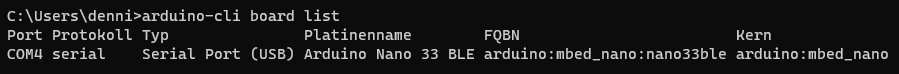
\includegraphics[width=11cm]{Arduino/CLI/boardlist.png}
        \caption{Rückgabewerte der \glqq board list\grqq-Funktion}
        \label{DBboardlist}
    \end{center}
\end{figure}

\begin{figure}[h]
    \begin{center}
        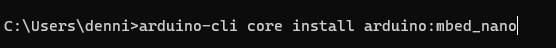
\includegraphics[width=11cm]{Arduino/CLI/KernInstallieren.png}
        \caption{Installieren des Kerns für den Arduino Nano 33 BLE Sense Lite}
        \label{KernInstallieren}
    \end{center}
\end{figure}


Zu Beginn sollte der richtige Kern für den Arduino Nano 33 BLE Sense Lite, wie in Abb. \ref{KernInstallieren} gezeigt, installiert werden. Dies erfolgt mit dem \glqq core install\grqq{}-Befehl und dem richtigen Kernnamen, der aus Abbildung \ref{DBboardlist} entnommen werden kann.


\subsection{Erstellung eines neuen Sketches}

Der erste Schritt ist die Erstellung eines neuen Sketches:

\medskip

\SHELL{arduino-cli sketch new cli\_test}

\medskip

Dieser Befehl erstellt ein Verzeichnis mit dem Namen \FILE{cli\_test}, die eine Datei mit dem gleichen Namen enthält.

\subsection{Kompilieren eines Sketches}

Die Funktion \glqq compile\grqq{} von \ac{cli} kann verwendet werden, um einen Sketch für jedes unterstützte Board zu kompilieren. Die entscheidende Option, die diese Funktion benötigt, ist der Board-Typ, der mit der Option \SHELL{--fqbn} angegeben werden kann. Die Abkürzung \SHELL{fqbn} bedeutet \glqq fully-qualified board name\grqq, was \glqq vollqualifizierter Board-Name\grqq{} bedeutet. Beispielsweise stehen folgende Boards zur Verfügung:


\begin{itemize}
    \item Arduino Uno: \SHELL{arduino:avr:uno}
    \item Arduino Mega: \SHELL{arduino:avr:mega}
    \item SparkFun RedBoard oder SparkFun BlackBoard: \SHELL{SparkFun:avr:RedBoard}; dies erfordert die zusätzliche Installation der Definition \glqq SparkFun avr board\grqq.
    \item  SparkFun SAMD21 Mini: \SHELL{SparkFun:samd:samd21\_mini}; dies erfordert die zusätzliche Installation der Definition \glqq SparkFun samd board\grqq.
    \Mynote{Portenta H7 und Nicla Vision fehlen}
\end{itemize}

Die möglichen Boards sind wie folgt aufgebaut:  \SHELL{manufacturer:architecture:board}.

\bigskip

Mit dem folgenden Kommando kann der Beispiel-Sketch, der sich im Ordner  \PATH{C:/Users/user.name/Documents/Arduino/} befindet, für einen Arduino UNO kompiliert werden.:

\medskip

\SHELL{arduino-cli compile --fqbn arduino:avr:uno C:/Users/user.name/Documents/Arduino/cli\_test}

\medskip

In der Abbildung \ref{ArduinoCompile} sieht man die Meldungen von \ac{cli}.

\begin{figure}
    \centering
    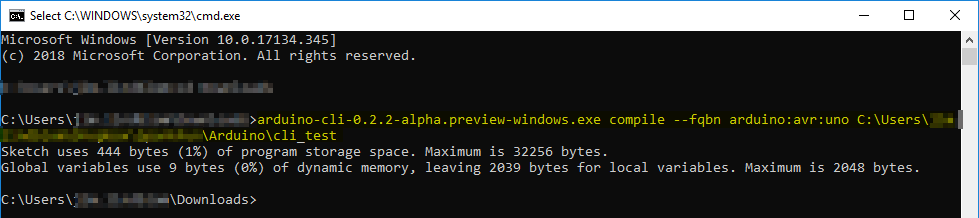
\includegraphics[width=\textwidth]{Arduino/arduino-cli-compile-cmd.png}
    \caption{Kompilieren eines Sketches mit \ac{cli}}
    \label{ArduinoCompile}
\end{figure}


Es können folgende Flags hinzugefügt werden:

\begin{itemize}
    \item Ausführlich \SHELL{-v}:  Nützlich, wenn alle Optionen und Dateien angezeigt werden sollen, die in Ihrem Sketch kompiliert werden.
    \item Build Pfad \SHELL{--build-path [string]}: Nützlich, wenn die kompilierten Objekt- und Hex-Dateien zu speichern sind. Auf meinem Windows-System muss der Wert dieses Parameters ein vollständiger Pfad sein.	
\end{itemize}

\subsection{Hochladen eines Sketches}

Ein kompilerter Sketch kann hochgeladen werden. Wie der Kompilierbefehl erfordert auch der Upload-Befehl eine \SHELL{--fqbn}. Außerdem wird eine serielle Schnittstelle zum Hochladen benötigt, die mit der Option \SHELL{-p} festgelegt wird.
Der folgende Befehl lädt den Beispiel-Sketch an einen Windows-COM-Anschluss auf COM18 hoch:

\medskip

\SHELL{arduino-cli upload -p COM18 --fqbn -v arduino:avr:uno C:/Users/user.name/Documents/Arduino/cli\_test}

\medskip


Falls es ordnungsgemäß durchgeführt wurde, sollte die RX/TX-LEDs des Arduinos zu blinken beginnen und kurz darauf einen leeren Sketch auszuführen.


\subsection{Installation von Bibliotheken}

Falls eine Bibliothek benötigt wird, so kann zunächst mit dem Kommando 

\medskip

\SHELL{arduino-cli lib search ethernet}

\medskip

on die Bibliothek, hier \SHELL{ethernet}, installiert ist. Mit dem Befehl

\medskip

\SHELL{arduino-cli lib install "{}UIPEthernet"}

\medskip

wird sie dann installiert.

\subsection{Beispiel \glqq Hello World\grqq}

Um das Kompilieren eines Sketches sowie das anschließende Hochladen mit Hilfe des Arduino-CLI zu demonstrieren, soll das \glqq Hello World!\grqq{}-Pendant für Mikrocontroller verwendet werden. Dafür wird ein einfacher Sketch, der die LED des Arduinos zum Blinken bringt, benutzt.

\begin{lstlisting}{Name}
    void setup(){
        pinMode(LED_BUILTIN, OUTPUT);
    }
    void loop(){
        digitalWrite(LED_BUILTIN, HIGH);
        delay(1000);
        digitalWrite(LED_BUILTIN, LOW);
        delay(1000);
    }
\end{lstlisting}

In der zu Beginn einmalig ausgeführten \SHELL{setup()}-Funktion wird die eingebaute \acs{led} als Output definiert \SHELL{pinMode(LED\_BUILTIN, OUTPUT)}. Dadurch lässt sich die LED später ansteuern. Innerhalb der \SHELL{loop()}-Funktion wird die LED zunächst eingeschaltet \SHELL{digitalWrite(LED\_BUILTIN, HIGH)} und mit einer Verzögerung von einer Sekunde \SHELL{delay(1000)} wieder abgeschaltet \SHELL{digitalWrite(LED\_BUILTIN}, \SHELL{LOW)}. Vor dem erneuten Einschalten der LED zu Beginn der Schleife wird am Schleifenende nochmal eine Sekunde gewartet um den blinkenden Effekt zu erzielen.

Um den Sketch zu kompilieren, kann der zuvor als Grundfunktion definierte Befehl \SHELL{compile}, wie in Abb. \ref{Kompilieren} dargestellt, verwendet werden.

\begin{figure}[h]
    \begin{center}
        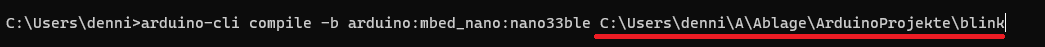
\includegraphics[width=11cm]{Arduino/CLI/Kompilieren.png}
        \caption{Für das Kompilieren des Blink-Sketches wird der Dateipfad zu dem Sketch mit angegeben (rot unterstrichen). Außerdem sollte der FQBN des Arduinos, für den der Sketch kompiliert wird, genannt werden.}
        \label{Kompilieren}
    \end{center}
\end{figure}

Anschließend kann der kompilierte Sketch mit Hilfe der \glqq upload\grqq{}-Funktion auf den Arduino hochgeladen werden. Dafür wird, wie in Abb. \ref{Hochladen} dargestellt, der Speicherpfad zu dem Sketch angegeben. Dadurch erfolgt das Hochladen der kompilierten Daten für den angegebenen Sketch.

\begin{figure}[h]
    \begin{center}
        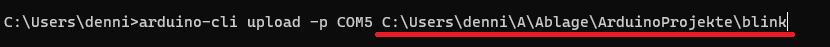
\includegraphics[width=11cm]{Arduino/CLI/Hochladen.png}
        \caption{Hochladen des kompilierten Sketches aus dem Temp-Ordner}
        \label{Hochladen}
    \end{center}
\end{figure}


Nach dem erfolgreichen Upload beginnt die in Abb. \ref{LEDtest} gezeigte LED des Arduino Nano 33 BLE Sense Lite zu blinken.

\begin{figure}[h]
    \begin{center}
        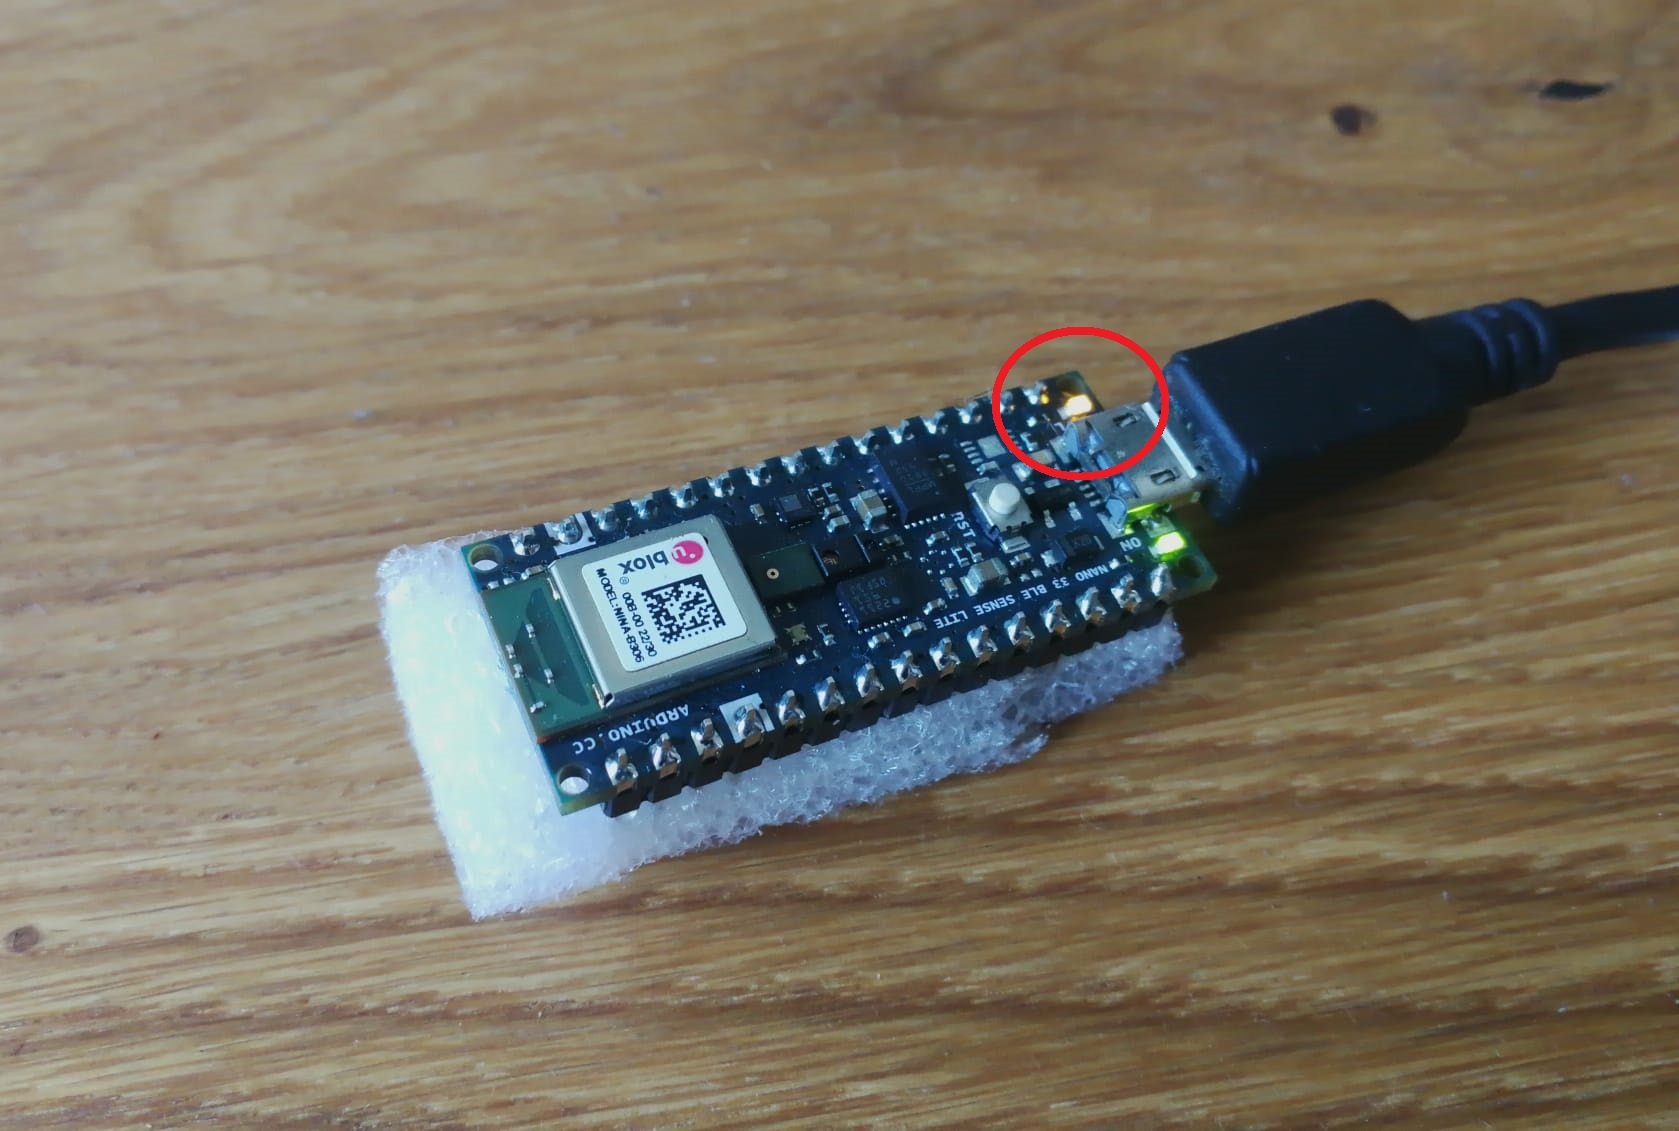
\includegraphics[width=11cm]{Arduino/CLI/LEDtesten.jpeg}
        \caption{Die orange LED des Arduinos beginnt zu blinken}
        \label{LEDtest}
    \end{center}
\end{figure}


\section{Beschreibung der Software auf dem PC}

Um einen erhöhten Automatisierungsgrad zu erreichen und die Potentiale des Arduino-CLI zu demonstrieren, wird ein Batch-Skript zum Testen der Sensoren verwendet. Dabei werden die Ergebnisse in einer Log-Datei dokumentiert. In diesem Abschnitt soll die Funktionsweise des Batch-Skriptes beschrieben werden.

{\small 
\begin{lstlisting}{Name}
@echo off
echo Logdatei Arduino-Setup, %time% Uhr, %date% > setup-log.txt
echo. >> setup-log.txt
echo. >> setup-log.txt
\end{lstlisting}
}

Mit dem Befehl \SHELL{\@echo off} wird die Ausgabe des Skript-Inhaltes bei Ausführung verhindert. Dadurch wird eine ansprechendere Frontend-Programmierung ermöglicht. In der zweiten Zeile wird die Log-Datei erstellt. Beim Erstellen wird mit der Überschrift \SHELL{Logdatei Arduino-Setup} sowie dem Auslesen der Systemzeit \SHELL{\%time\%} und des Datums \SHELL{\%date\%} die erste Zeile des Protokolls versehen. Für die spätere Übersichtlichkeit der Log-Datei folgen zwei leere Zeilen \SHELL{echo. >> setup-log.txt}. Mit dem einmaligen Anwenden des größer als Operators \SHELL{> setup-log.txt} wird eine neue Datei erstellt oder eine Bestehende mit dem gleichen Namen überschrieben. Bei doppelter Anwendung des größer als Operators \SHELL{>> setup-log.txt} wird der linksseitige Inhalt in einer neuen Zeile an eine bestehende Datei angehängt. So wird die Log-Datei Zeile für Zeile beschrieben und nicht einmalig komplett am Ende des Batch-Skriptes.

\begin{lstlisting}{Name}
:: Gegebenenfalls wird der Kern installiert
echo Kernstatus: >> setup-log.txt
arduino-cli core install arduino:mbed_nano >> setup-log.txt
\end{lstlisting}

Kommentare in dem Batch-Skript werden durch zwei aufeinanderfolgende Doppelpunkte gekennzeichnet \SHELL{:: Gegebenenfalls wird der Kern installiert} und sollen die Nachvollziehbarkeit innerhalb des Skriptes erhöhen. Mit dem Befehl \SHELL{echo Kernstatus: >> setup-log.txt} wird in der Log-Datei gekennzeichnet, dass in der nächsten Zeile Informationen über den zu installierenden Kern für den Arduino Nano 33 BLE Sense Lite folgen. Das Arduino-CLI bringt bereits die Intelligenz mit zu prüfen, ob der angegebene Kern schon installiert ist. Sollte dies der Fall sein, erfolgt die entsprechende Dokumentation in der Log-Datei. Das Installieren des Kerns wird mit der Zeile \SHELL{arduino-cli core install arduino:mbed\_nano >> setup-log.txt} initialisiert. Dabei ist der für den Arduino Nano 33 BLE Sense Lite notwendige Kern mit dem Namen \SHELL{arduino:mbed\_nano} angegeben. Der Rückgabewert der Funktion zum Kerninstallation wird in der Log-Datei gespeichert.

\begin{lstlisting}{Name}
echo Es wird nach angeschlossenen Boards gesucht...
:: Auflisten der angeschlossenen Arduinos
echo Folgende Boards sind am PC angeschlossen: >> setup-log.txt
echo.
echo. >> setup-log.txt
arduino-cli board list >> setup-log.txt
arduino-cli board list
echo.
\end{lstlisting}

Zu Beginn dieses Skript-Abschnittes wird zunächst der Nutzer der Software über die Suche nach den angeschlossenen Arduino Platinen informiert \SHELL{echo Es wird nach angeschlossenen Boards gesucht...}. Folgend wird mit dem Befehl \SHELL{echo Folgende Boards sind am PC angeschlossen: >> setup-log.txt} über den Inhalt der nächsten Zeile in der Log-Datei informiert. Die Information darüber welche Arduinos an dem PC angeschlossen sind, kann mit dem Befehl \SHELL{arduino-cli board list}, der hier doppelt ausgeführt wird, gewonnen werden. Bei der ersten Ausführung wird die Rückgabe des Arduino-CLI in der Log-Datei gespeichert \SHELL{>> setup-log.txt}, die zweite Ausführung dient zur Anzeige in dem aktuell ausgeführten Skript. Die Information über die angeschlossenen Arduinos benötigt der Nutzer im nächsten Schritt für eine Eingabe.

\begin{lstlisting}{Name}
:: Abfragen des Portnamens fuer spaeteren Upload 
:: der Sensorentestdatei
set /p port="Bitte den Portnamen des Sense-Lite eingeben und bestaetigen: "
echo Der Port %port% wurde gewaehlt. >> setup-log.txt
\end{lstlisting}

In der Zeile \SHELL{set /p port="Bitte den Portnamen des Sense-Lite eingeben und bestaetigen: "} erfolgt eine Nutzerabfrage. Der Befehl \SHELL{set} ermöglicht das Setzen der Variable \SHELL{port} auf einen bestimmten Wert. Mit dem Zusatz \SHELL{/p} wird dieser bestimmte Wert auf die folgende Nutzereingabe gesetzt. Die Ausführung des Skriptes wird bis zur erfolgreichen Eingabe des Nutzers gestoppt. Die Nutzereingabe beinhaltet den Port des angeschlossenen Arduino Nano 33 BLE Sense Lite. Für die spätere Nachvollziehbarkeit wird der gewählte Port in der Log-Datei mit der Zeile \SHELL{echo Der Port \%port\% wurde gewaehlt. >> setup-log.txt} dokumentiert. 

\begin{lstlisting}{Name}
:: Anlegen des Ordners fuer den kompilierten Sensorentest
set ordner=SensorentestCompiledData
mkdir %ordner%
\end{lstlisting}

Die Variable \SHELL{ordner} bekommt den Wert \SHELL{SensorentestCompiledData} zugewiesen. In der nächsten Zeile \SHELL{mkdir \%ordner\%} wird der Ordner mit dem Namen \PYTHON{SensorentestCompiledData} für das spätere Speichern des kompilierten Sketches angelegt.

\begin{lstlisting}{Name}
:: Gegebenenfalls werden die noetigen Bibliotheken fuer 
:: den Sensorentest installiert
:: Bib fuer IMU
echo Bib fuer IMU >> setup-log.txt
arduino-cli lib install Arduino_LSM9DS1 >> setup-log.txt
echo. >> setup-log.txt
    
:: Bib fuer Farbsensor
echo Bib fuer Farbsensor >> setup-log.txt
arduino-cli lib install Arduino_APDS9960 >> setup-log.txt
echo. >> setup-log.txt
    
:: Bib fuer Druck- und Temperatursensor
echo Bib fuer Druck- und Temperatursensor >> setup-log.txt
arduino-cli lib install Arduino_LPS22HB >> setup-log.txt
echo. >> setup-log.txt
\end{lstlisting}

In der Log-Datei wird jeweils dokumentiert um welche Bibliothek es sich in der folgenden Zeile handelt \SHELL{SensorentestCompiledData}. Anschließend erfolgt mit dem Befehl \SHELL{arduino-cli lib install Arduino\_LSM9DS1 >> setup-log.txt} das Installieren der Bibliothek sowie das Speichern des Rückgabewertes der Installation in der Log-Datei. Eine bereits installierte Bibliothek wird von dem Arduino-CLI erkannt und es folgt eine entsprechende Rückgabe in die Log-Datei. Das Vorgehen ist für alle drei zu installierenden Bibliotheken identisch.

\begin{lstlisting}{Name}
:: Kompilieren des Sensorentest-Sketches
echo Kompilieren des Sensorentest-Sketches: >> setup-log.txt
echo. >> setup-log.txt
arduino-cli compile -b arduino:mbed_nano:nano33ble %cd%\SensortestLite 
--build-path %cd%\%ordner% >> setup-log.txt
\end{lstlisting}

Nachdem die notwendigen Bibliotheken installiert sind, kann der zuvor erstellte Sketch zum Testen der Sensoren kompiliert werden. Das Kompilieren des Sketches für den Arduino Nano 33 BLE Sense Lite erfolgt mit dem Befehl \SHELL{arduino-cli compile -b arduino:mbed\_nano:nano33ble \%cd\%/SensortestLite}. Der hintere Teil des Befehls gibt den Speicherpfad des zu kompilierenden Sketches an. Weiterhin lässt sich der Zielordner für den kompilierten Sketch mit dem Zusatz \SHELL{--build-path \%cd\%/\%ordner\% >> setup-log.txt} definieren. Der Rückgabewert des Kompilierens mit dem Arduino-CLI wird in der Log-Datei gespeichert.

\begin{lstlisting}{Name}
:: Hochladen des kompilierten Sketches auf den Arduino
echo Hochladen des kompilierten Sketches auf den Arduino >> setup-log.txt
arduino-cli upload -p %port% --input-dir %cd%\%ordner% >> setup-log.txt
\end{lstlisting}

Der kompilierte Sketch wird in der Zeile \SHELL{arduino-cli upload -p \%port\% --input-dir}  \SHELL{\%cd\%/\%ordner\% >> setup-log.txt} auf den durch \SHELL{port} angeschlossenen Arduino Nano 33 BLE Sense Lite hochgeladen. Der Speicherpfad der kompilierten Daten wird mit dem Zusatz \SHELL{--input-dir \%cd\%/\%ordner\%} angegeben.

\begin{lstlisting}{Name}
:: Oeffnen des seriellen Monitors
start monitor_log
:: Automatisches Schlieszen des seriellen Monitors nach 4 Sekunden 
:: (n-1 Sekunden, mit n=5)
ping 127.0.0.1 -n 5 > nul
taskkill /im serial-monitor.exe /F
\end{lstlisting}

Mit dem Befehl \SHELL{start monitor\_log} wird ein weiteres Batch-Skript zum Auslesen des seriellen Monitors aufgerufen. Die Zeile \SHELL{ping 127.0.0.1 -n 5 > nul} stoppt die Ausführung der Software für vier Sekunden. Dabei werden fünf Anfragen an den lokalen Rechner gesendet und jeweils eine Sekunde zwischen zwei Anfragen gewartet. Mit \SHELL{> nul} wird die Ausgabe der Antworten ins Leere geleitet und nicht angezeigt. Ist die Zeitspanne von vier Sekunden abgelaufen wird der serielle Monitor zum Auslesen der Sensordaten automatisch mit dem Befehl \SHELL{taskkill /im serial-monitor.exe /F} geschlossen. Über den Zusatz \SHELL{/im} kann das zu schließende Fenster \SHELL{serial-monitor.exe} benannt werden. Das erzwungene Schließen des seriellen Monitors erfolgt mit dem Anhang \SHELL{/F}. Nachdem der serielle Monitor ausgelesen und geschlossen wurde, kann die Software beendet werden. Die Ergebnisse des Sensoren-Tests lassen sich im Anschluss der Log-Datei entnehmen.

Das Öffnen des seriellen Monitors erfolgt in dem Skript \FILE{monitor\_log.bat}.

\begin{lstlisting}{Name}
echo Sensordaten: >> setup-log.txt
echo. >> setup-log.txt
    
echo Der serielle Monitor wird geoeffnet, die Sensordaten werden ausgelesen und in der Logdatei gespeichert...
    
arduino-cli monitor -p %port% >> setup-log.txt
\end{lstlisting}	

Der serielle Monitor kann mittels des Arduino-CLI Befehls \SHELL{arduino-cli monitor} \SHELL{-p \%port\% >> setup-log.txt} geöffnet werden. Dabei wird mit \SHELL{-p \%port\%} die Verbindung für den angegebenen Port hergestellt. Mit dem Zusatz \SHELL{>> setup-log.txt} werden die empfangenen Daten in die Log-Datei geschrieben.
